\section{CRUD, Express et MongoDB}
\paragraph{CRUD}C'est un acronym pour \textbf{CREATE}, \textbf{READ}, \textbf{UPDATE} et \textbf{DELETE} dans certaines denomition il existe un dernier element \textbf{EXECUTE}. C'est une liste d'operation que l'on demande au serveur d'executer au travers des requêtes \textbf{POST}, \textbf{GET}, \textbf{PUT} et \textbf{DELETE} respectivement.
\begin{center}
	\makebox[\textwidth]{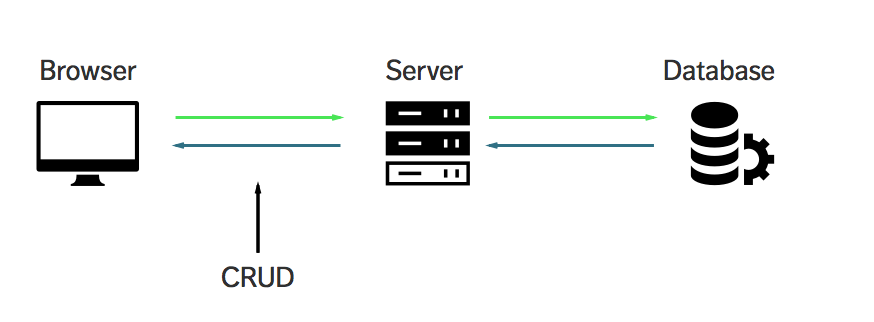
\includegraphics[width=\textwidth]{./media/crud-express-mongo.png}}
\end{center}
\subsection{}